
\chapter{Computing Performance of sequential code\label{chpt:seq-code-performance}}

This section evaluates the computing performance of the code without
parallelization. Our goal is to show that the new algorithm of angular
convolution is faster than the old naive one, and the huge amount
of simulation has shown that it is absolutely the case. But a raw
result, where the implementation goes for an indefinite number of
iterations during minimization, cannot give a proper and systematic
performance evolution. This gives the propose of this section. 

As discussed in appendix \ref{chpt:computing-performance}, two main
factors give influence to the performance of a sequential code: the
algorithm complexity, and the memory delay. To study the algorithm
complexity, testing with respect to parameters is done to some simple
but important components. The result can match the theoretical algorithm
complexity, or completely different due to the overhead of function
calling or the inhomogeneity of memory access. Etude of this small
parts permits a further understanding of the entire code.


\section{FFT}

The \acs{FFT} play a great role in the implementation, which is used
by the spatial convolution and the \acs{FGSHT} process. As shown
in figure \ref{fig:timing-FFT}a, the dependance on $O(N\log_{2}N)$
doesn't totally exist, due to the algorithm of FFT {[}ref dft{]}.
To compare between the algorithms involved in this thesis, we are
not really interested in computing performance with respect to the
number of spatial grid, but the \acs{FFT} used in \acs{FGSHT} process
(figure \ref{fig:timing-FFT}b). 

\begin{figure}[h]
\subfloat[spatial+nlogn!]{\begin{centering}
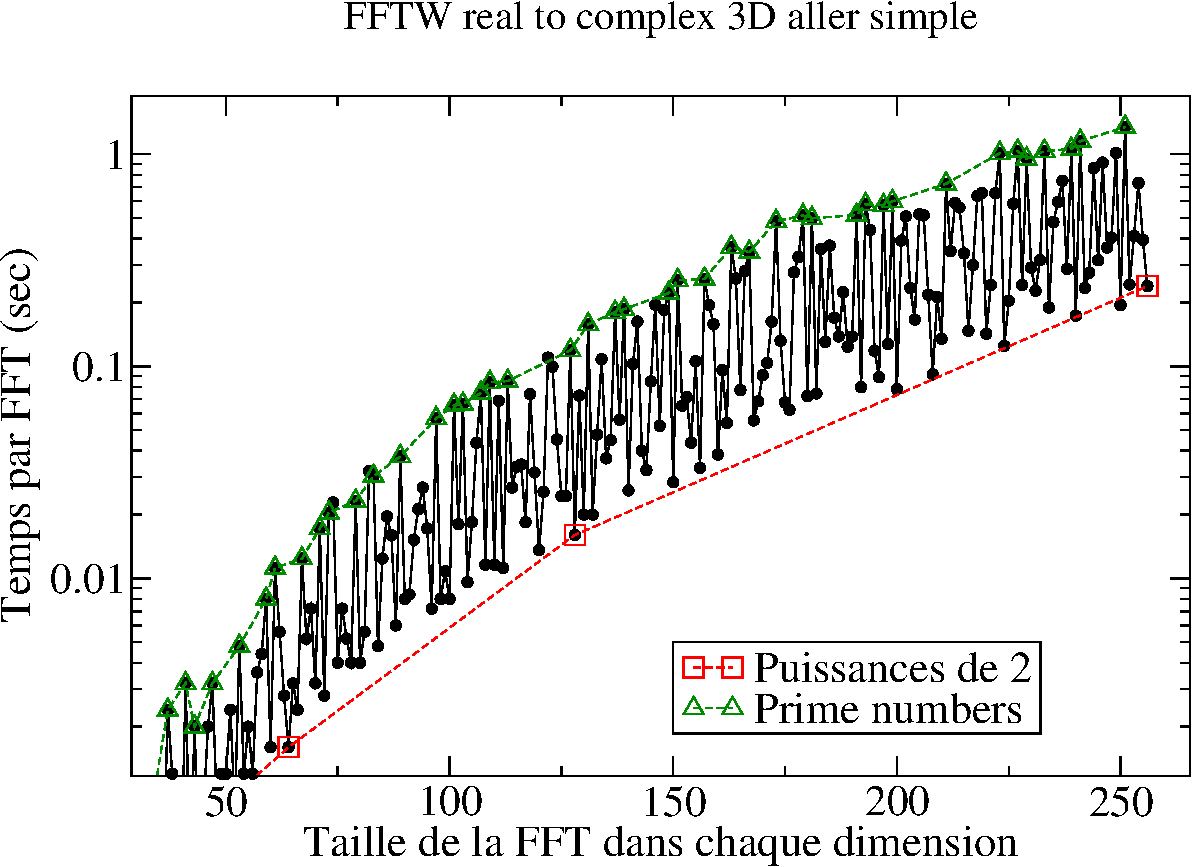
\includegraphics[width=0.5\columnwidth]{_figure/timing_fft_spatial}
\par\end{centering}

}\subfloat[angular]{}

\caption{timing FFT\label{fig:timing-FFT}}
\end{figure}



\section{FGSHT}


\subsection{Computing time of GSHT and FGSHT}

To serve as an alternative of FFT for angular grid, the algorithmic
complicity of GSHT should be at least less than $O(N_{\mathbf{\Omega}}^{2})$,
where $N_{\mathbf{\Omega}}$ is the total number of Euler angles.
But to integrate eq. (\ref{eq:gsht-fwd}) in a direct way, $(n+1)(2n+1)(2\left\lfloor n/s\right\rfloor +1)=N_{\Theta}N_{\Phi\Psi}=N_{\mathbf{\Omega}}$
function evaluations (FE) are needed for each $F_{\mu'\mu}^{m}$ ($s=1$
or 2 according to the symmetry of axe $\mathrm{C}_{s}$), an overall
$O(N_{\mathbf{\Omega}}^{2})$ process is needed and \textit{vice versa}.
A faster algorithm proposed by Numerical Recipes \citep{Numerical_Recipes_3ed}
suggests reducing this cost to $O(N_{\Theta}^{2}N_{\Phi\Psi}\ln N_{\Phi\Psi}\simeq N_{\mathbf{\Omega}}^{4/3})$
by FFT. The implementation is detailed in appendix \ref{chpt:fgsht-via-fft}.
The computing time of GSHT and FGSHT are shown in figure \ref{fig:time-gsht-fgsht},
for the case that $\Psi$ possesses no symmetry.

It is shown that the computing cost reduced by FFT is about ... times
of the original cost, which is agreed with the prediction. ? 

\begin{figure}[h]
\caption{Computing time of GSHT and FGSHT (per 1000 times)\label{fig:time-gsht-fgsht}}
\end{figure}



\subsection{Performance with respect to $m_{\max}$}


\subsection{Performance with respect to $n_{\max}$}

psi treatment for mmax/nmax different


\section{K-kernel}


\subsection{Comparison between paths}

Timing paths in figure \ref{fig:k-kernel}


\subsection{$m_{\max}$ and $n_{\max}$ dependance of OZ equation}

Theoretical listed in table \ref{tab:FE-of-OZ}. 

with respect to nmax


\section{Entire iteration of $\mathcal{F}_{\mathrm{exc}}$ evaluation}


\subsection{Comparison between ``naive\_standard'' and ``convolution\_pure\_angular''}

\begin{figure}[h]
\caption{}
\end{figure}


difference after FFT.

verified the conclusion of k-kernel test.


\subsection{Comparison between ``convolution\_standard'' and ``convolution\_asymm''}

\begin{figure}[h]
\caption{}
\end{figure}


The symmetries, ideally the time should be reduced by two, but as
shown in $\mathsection$, convolution\_standard need more ``decoration''.


\subsection{Comparison between ``convolution\_standard'' and ``convolution\_pure\_angular''}

\begin{figure}[h]
\caption{}
\end{figure}


The inversion of FFT and FGSHT

we can see the other part is almost identical, but the implementation
of FFT takes different time. Because in convolution\_standard the
number of FE we need for FFT is the number of projections, and in
convolution\_pure\_angular it is the number of angular grid nodes.
As there is less projections than angular nodes, convolution\_standard
reasonably takes less time.


\section{Global view of the sequential code performance}

Computing time and memory limits

Hotspots and bottlenecks
